\documentclass[english,serif,mathserif,xcolor=pdftex,dvipsnames,table]{beamer}
\usepackage{gc3}

\title{%
  The \texttt{StagedTaskCollection}
}
\author[Riccardo Murri]{%
  GC3: Grid Computing Competence Center, \\
  University of Zurich
}
\date{Oct.~2, 2012}

\begin{document}

% title frame
\maketitle


\begin{frame}[fragile]
  \frametitle{Running jobs in sequence}

  \texttt{StagedTaskCollection} provides a simplified interface for
  constructing sequences of jobs, but it only applies when the number
  and content of steps is \emph{known and fixed} at programming time.

  \+ 
  (By contrast, the most general \texttt{SequentialTaskCollection}
  can alter the sequence on the fly, insert new stages while running
  and loop back. But the code is also harder to write.)
\end{frame}


\begin{frame}[fragile]
  \begin{columns}[t]
    \begin{column}{0.6\textwidth}
      \begin{lstlisting}
class Pipeline@\HL{(StagedTaskCollection)}@:
  def __init__(self, image):
    self.source = image

  def stage0(self):
    # run 1st step
    return Application(...)

  def stage1(self):
    if self.tasks[0].execution.exitcode != 0:
      self.execution.exitcode = 1
      return Run.State.TERMINATED
    else:
      # run 2nd step
      return Application(...)

  # ...
  def stage@$N$@(self):
    # ...
      \end{lstlisting}
    \end{column}
    \begin{column}{0.4\textwidth}
      \raggedleft

      \+\+
      Example of~a \texttt{StagedTaskCollection}
      subclass.
    \end{column}
  \end{columns}
\end{frame}


\begin{frame}[fragile]
  \begin{columns}[c]
    \begin{column}{0.6\textwidth}
      \begin{lstlisting}
class Pipeline(StagedTaskCollection):
  def __init__(self, image):
    self.source = image

  def @\HL{stage0(self)}@:
    # ...

  def @\HL{stage1(self)}@:
    # ...

  # ...
  def @\HL{stage$\mathbf N$(self)}@:
    # ...
      \end{lstlisting}
    \end{column}
    \begin{column}{0.4\textwidth}
      \raggedleft

      Stages are numbered starting from $0$.

      \+
      You can have as many stages as you want.
    \end{column}
  \end{columns}
\end{frame}


\begin{frame}[fragile]
  \begin{columns}[c]
    \begin{column}{0.6\textwidth}
      \begin{lstlisting}
class Pipeline(StagedTaskCollection):
  # ...

  def stage0(self):
    # run 1st step
    @\HL{return Application}@(
      ['convert', self.source, 
       '-colorspace', 'gray',
       'grayscale_' + self.source],
      inputs = [self.source],
      ...)

  # ...
      \end{lstlisting}
    \end{column}
    \begin{column}{0.4\textwidth}
      \raggedleft 

      Each \texttt{stage$N$} method can return a \texttt{Task}
      instance, that will run as step $N$ in the sequence.
    \end{column}
  \end{columns}
\end{frame}


\begin{frame}[fragile]
  \begin{columns}[c]
    \begin{column}{0.6\textwidth}
      \begin{lstlisting}
class Pipeline(StagedTaskCollection):
  # ...

  def stage1(self):
    @\HL{if self.tasks[0].execution.exitcode != 0:}@
      self.execution.exitcode = 1
      return Run.State.TERMINATED
    else:
      # run 2nd step
      return Application(...)

  # ...
  def stage@$N$@(self):
    # ...
      \end{lstlisting}
    \end{column}
    \begin{column}{0.4\textwidth}
      \raggedleft

      \+\+\+\+\+ 
      In later stages you can check the exit code of
      earlier ones, and decide whether to continue the sequence or
      abort.
    \end{column}
  \end{columns}
\end{frame}


\begin{frame}[fragile]
  \begin{columns}[c]
    \begin{column}{0.6\textwidth}
      \begin{lstlisting}
class Pipeline(StagedTaskCollection):
  # ...

  def stage1(self):
    if self.tasks[0].execution.exitcode != 0:
      self.execution.exitcode = 1
      @\HL{return Run.State.TERMINATED}@
    else:
      # run 2nd step
      return Application(...)

  # ...
  def stage@$N$@(self):
    # ...
      \end{lstlisting}
    \end{column}
    \begin{column}{0.4\textwidth}
      \raggedleft

      \+\+\+\+\+
      To abort the sequence, return \texttt{Run.State.TERMINATED},
      instead of a \texttt{Task} instance.
    \end{column}
  \end{columns}
\end{frame}


\begin{frame}[fragile]
  \begin{columns}[c]
    \begin{column}{0.6\textwidth}
      \begin{lstlisting}
class Pipeline(StagedTaskCollection):
  # ...

  def stage1(self):
    if self.tasks[0].execution.exitcode != 0:
      @\HL{self.execution.exitcode = 1}@
      return Run.State.TERMINATED
    else:
      # run 2nd step
      return Application(...)

  # ...
  def stage@$N$@(self):
    # ...
      \end{lstlisting}
    \end{column}
    \begin{column}{0.4\textwidth}
      \raggedleft

      \+\+\+\+\+
      Don't forget to set the \texttt{StagedTaskCollection}'s own exit
      code if you do this.
    \end{column}
  \end{columns}
\end{frame}


\begin{frame}[fragile]
  \frametitle{Detour: grayscaling an image}
  The \href{http://www.imagemagick.org}{ImageMagick}
  command to reduce an image to grayscale is:
  \begin{lstlisting}[language=sh]
    $ convert @\emph{image1}@ -colorspace gray @\emph{image2}@
  \end{lstlisting}%$
  
  \+ 
  It reads the image in file \emph{image1}, converts it to a
  black\&white picture, and saves the result into file \emph{image2}.

  \+
  \begin{tabular}[c]{ccc}
    
\includegraphics[width=0.4\textwidth]{fig/lena}
    &
    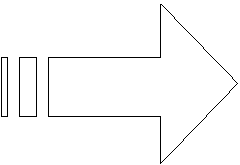
\includegraphics[width=0.1\textwidth]{fig/arrow}
    &
    
\includegraphics[width=0.4\textwidth]{fig/lena_gray}
  \end{tabular}
\end{frame}


\begin{frame}[fragile]
  \frametitle{Detour: inverting colors}
  The \href{http://www.imagemagick.org}{ImageMagick}
  command to invert colors is:
  \begin{lstlisting}[language=sh]
    $ convert @\emph{image1}@ +negate @\emph{image2}@
  \end{lstlisting}%$
  
  \+ 
  It reads the image in file \emph{image1}, inverts colors (black
  $\to$ white and reverse), and saves the result into file
  \emph{image2}.

  \+
  \begin{tabular}[c]{ccc}
    
\includegraphics[width=0.4\textwidth]{fig/lena_gray}
    &
    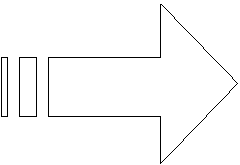
\includegraphics[width=0.1\textwidth]{fig/arrow}
    &
    
\includegraphics[width=0.4\textwidth]{fig/lena_negative}
  \end{tabular}
\end{frame}


\begin{frame}[fragile]
  \frametitle{Detour: mounting images side-by-side}
  The \href{http://www.imagemagick.org}{ImageMagick}
  command to invert colors is:
  \begin{lstlisting}[language=sh]
    $ montage @\emph{image1}@ @\emph{image2}@ -tile 2x1 @\emph{image3}@
  \end{lstlisting}%$
  
  \+ 
  It reads files \emph{image1} and \emph{image2}, creates a
  combined picture by putting the two side-by-side\footnote{a tile
    with $2$ columns by $1$ row} and saves the result into file
  \emph{image3}.

  \+
  \begin{tabular}[c]{ccc}
    
\includegraphics[width=0.3\textwidth]{fig/lena_gray}
    \hspace{-0.2\textwidth}\raisebox{-0.1\textwidth}{
\includegraphics[width=0.3\textwidth]{fig/lena_negative}}
    &
    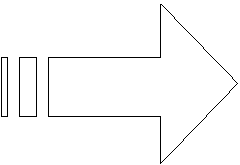
\includegraphics[width=0.1\textwidth]{fig/arrow}
    &
    
\includegraphics[width=0.4\textwidth]{fig/lena2x1}
  \end{tabular}
\end{frame}


\begin{frame}[fragile]
  \begin{exercise}
    Write a \emph{SideBySide} sequence. 

    \+ 
    The sequence is initialized with the file name of a picture:
    \begin{lstlisting}
      sbs = SideBySide('fig/lena.jpg')
    \end{lstlisting}

    \+
    The sequence runs the following steps on the input image:
    \begin{enumerate}
    \item Convert it to grayscale.
    \item Invert colors in the grayscale picture.
    \item Mount the two images side by side and write them into a final output image.
    \end{enumerate}

    \+ 
    Plug this class into your standard session based script and
    verify that it works.
  \end{exercise}
\end{frame}


\end{document}

%%% Local Variables: 
%%% mode: latex
%%% TeX-master: t
%%% End: 
